% \documentclass[aspectratio=169]{beamer}
% \mode<presentation>

\documentclass[aspectratio=169]{beamer}
% \documentclass[aspectratio=169,handout]{beamer}
\usepackage{pgfpages}
\mode<presentation>
\setbeameroption{show notes}
% \setbeameroption{show notes on second screen=right}
\setbeamertemplate{note page}[compress]
% \pgfpagesuselayout{6 on 1}[letterpaper,border shrink=5mm]
% \pgfpagesuselayout{4 on 1}[letterpaper,landscape,border shrink=5mm]



%Theme and Color of Presentation
\usetheme{CambridgeUS}
\usecolortheme{seahorse}
\useinnertheme{rectangles}

%Colors
% From https://www.utdallas.edu/brand/color-palette/
\definecolor{UTDorange}{RGB}{232,117,0}
\definecolor{UTDgreen}{RGB}{18,71,52}
\definecolor{UTDseafoam}{RGB}{95,244,183}

\setbeamercolor{palette primary}{bg=UTDorange,fg=white}
\setbeamercolor{palette secondary}{bg=UTDgreen,fg=white}
\setbeamercolor{palette tertiary}{bg=UTDorange,fg=white}
\setbeamercolor{palette quaternary}{bg=UTDorange,fg=white}
\setbeamercolor{frametitle}{fg=UTDgreen}
\setbeamercolor{structure}{fg=UTDgreen} % itemize, enumerate, etc
\setbeamercolor{subsection in head/foot}{bg=UTDgreen,fg=white}


%Additional Packages
\usepackage{graphicx}
\usepackage{physics}
\usepackage{amsmath}
\usepackage{setspace}
\usepackage{textpos}
\usepackage{hyperref}
\usepackage{xcolor}
% \usepackage{enumitem}

%Additional Settings/Commands
\newcommand{\extraspace}{\vskip 0.5em}

\AtBeginSection[]
{
	\begin{frame}<beamer>[noframenumbering]
		\frametitle{Outline}
		\tableofcontents[currentsection]
	\end{frame}
}
\AtBeginSubsection[]
{
	\begin{frame}<beamer>[noframenumbering]
		\frametitle{Outline}
		\tableofcontents[currentsection,currentsubsection]
	\end{frame}
}

%Presentation Info
\title[2nd-order System Dynamics]{Introduction to 2\textsuperscript{nd}-order System Response}
\author{Jonas Wagner}
\institute[UTDallas]{The University of Texas at Dallas}
\date{}

\begin{document}
	
\begin{frame}
	\titlepage
\end{frame}

\addtobeamertemplate{frametitle}{}{%
	\begin{textblock*}{100mm}(.85\textwidth,-1cm)
		
\includegraphics[height=1cm]{Images/UT_Dallas_Logo}
	\end{textblock*}
}

\begin{frame}{Outline}
	\tableofcontents
	\note{
		4th-wall break notes
		\begin{itemize}
			\item Lecture Objective:
			% \begin{itemize}
				% \item 
				\textbf{why 2nd-order roots of a dynamical system's can result in more interesting responses}
				(i.e.) the 3 cases as a result from the quadratic equation
			% \end{itemize}
			\item Math background/assumptions:
			\begin{itemize}
				\item Simple ODEs solutions are covered in prereq and explained again in the intro of this course
				\item Specifically, Laplace transform methods and the \textbf{inverse-laplace via partial fraction expansion} will be well known to students. 
				\item In a real course I'd spend time in lecture having students walk me through the derivation of the cases instead of leaving as an exercise/assignment.
			\end{itemize}
			\item Previous lectures:
			\begin{itemize}
				\item 1st order-system response and how time-constant plays into the system impulse and step-response
				\item Solutions to differential equations (w/in time and frequency domains)
			\end{itemize}
		\end{itemize}
	}
\end{frame}

\section{Motivation}
\begin{frame}
	\frametitle{Real-World Dynamical Systems}
	\begin{columns}
		\begin{column}{0.6\linewidth}
			\centering
			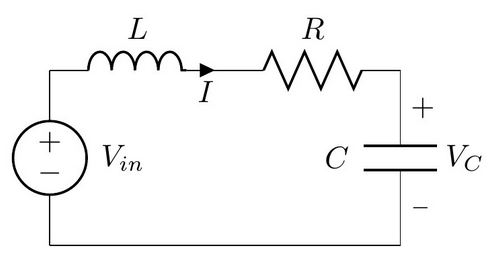
\includegraphics[width=0.5\textwidth]{Images/LCR_circuit.png}\\
			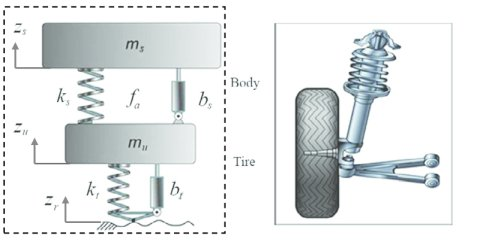
\includegraphics[width=0.9\textwidth]{Images/car_supension.jpg}
		\end{column}
		\begin{column}{0.3\linewidth}
			\centering
			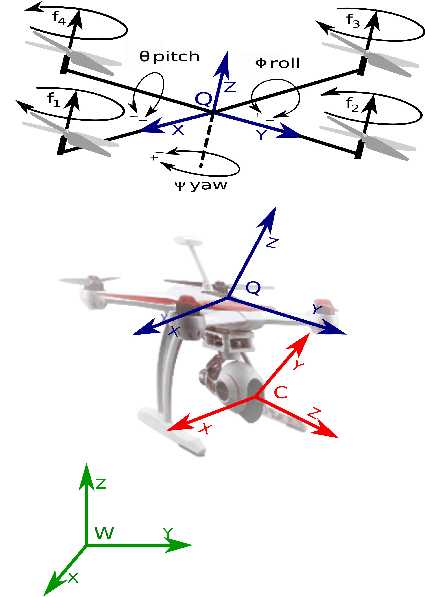
\includegraphics[width=0.9\textwidth]{Images/Quadcopter-model-and-the-coordinate-systems-relationship.png}
		\end{column}
	\end{columns}
\end{frame}

\section{Forced Response}
\begin{frame}
	\frametitle{Step Response - 1st vs 2nd order}
	\begin{itemize}[<+->]
		\item[] \textbf{Step Input:}
			$\textbf{u}(t) \overset{\mathcal{L}}{\Rightarrow} U(s) = \frac{1}{s}$\\
		\item[] \textbf{1\textsuperscript{st}-order:}
		\[
			Y(s) = \frac{K}{\alert<.(3)>{\tau s + 1}} \qty(\frac{1}{s})
			\quad \overset{\mathcal{L}^{-1}}{\Rightarrow} \quad
			y(t) = K (1 \alert<.(3)>{- e^{-t/\tau}}) \mathbf{u}(t)
		\]
		\only<+| handout:0>{\begin{center}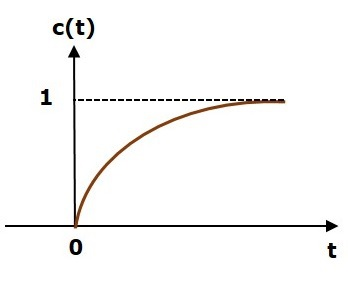
\includegraphics[width = 0.3\textwidth]{Images/step_response_1st.jpg}\end{center}}
		\item[] \textbf{2\textsuperscript{nd}-order:}
		\[
			Y(s) = \frac{K}{\alert<+->{(s+p_1)(s+p_2)}} \qty(\frac{1}{s})
			% = \frac{C_1}{s} + \frac{C_2}{s+p_1} + \frac{C_3}{s+p_2}
			\quad \overset{\mathcal{L}^{-1}}{\Rightarrow} \quad
			y(t) = \qty(C_1 + \alert<.->{C_2 e^{-p_1 t} + C_3 e^{-p_2 t}}) \mathbf{u}(t)
		\]
	\end{itemize}
	\only<.| handout:0>{\begin{center}
		\alert{$\Delta(s)$ dictates transient dynamics}
	\end{center}}
	\only<+->{\begin{columns}
		\begin{column}{0.4\textwidth}
			\textbf{3 distinct cases:}
			\begin{itemize}
				\item<.-> Damped: \alert{$p_1 \neq p_2$}
				\item<+-> Critically Damped: \alert{$p_1 = p_2$}
				\item<+-> Underdamped: \alert{$p_{1,2} = \sigma \pm j \omega$}
			\end{itemize}
		\end{column}
		\begin{column}{0.4\textwidth}
			\centering
			\only<.(-2)| handout:0>{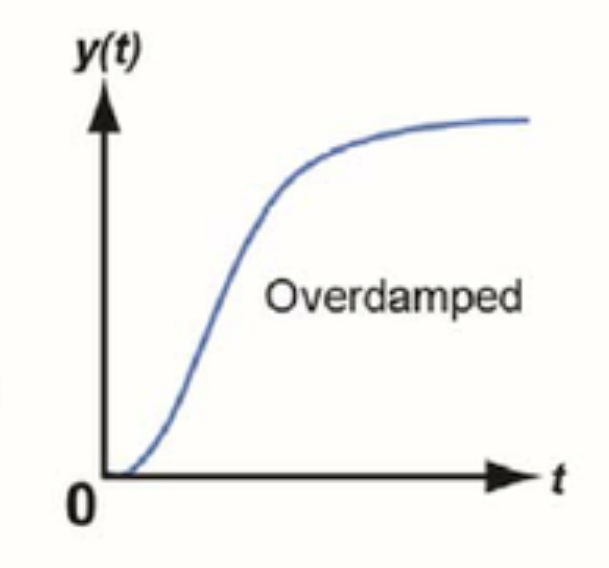
\includegraphics[width=0.5\columnwidth]{Images/step_response_2nd_overdamped.png}}
			\only<.(-1)| handout:0>{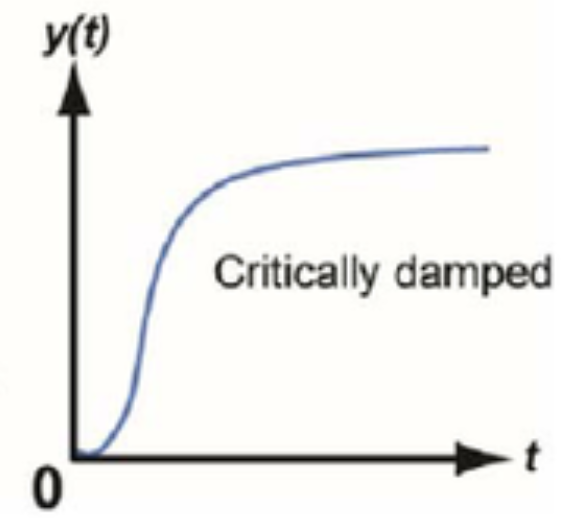
\includegraphics[width=0.5\columnwidth]{Images/step_response_2nd_critdamped.png}}
			\only<.| handout:0>{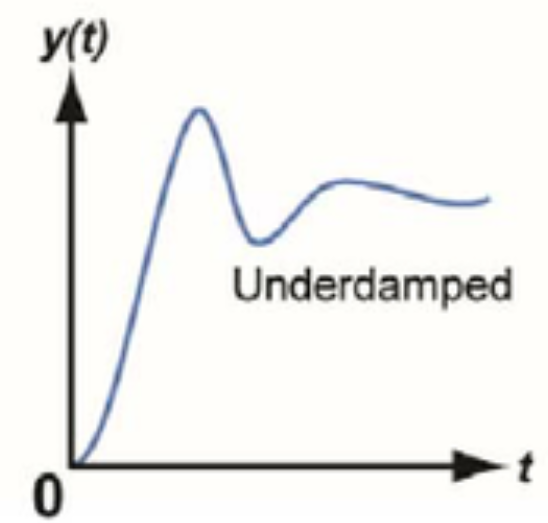
\includegraphics[width=0.5\columnwidth]{Images/step_response_2nd_underdamped.png}}
			\only<+->{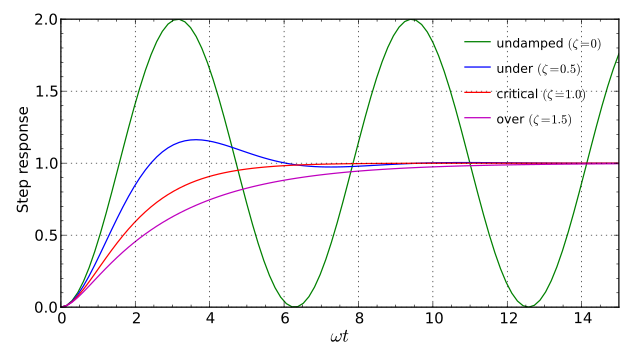
\includegraphics[width=\columnwidth]{Images/step_response_2nd.png}}
		\end{column}
	\end{columns}}
\end{frame}

\section{Applied Example: Spring-Mass-Damper}
\subsection{Review: System Modeling}
\begin{frame}
	\frametitle{Spring Mass-Damper System Modeling}
	\begin{columns}
		\begin{column}{0.5 \textwidth}
			Newton's 2\textsuperscript{nd} Law:
			\[
				F = m \vb{a} 
				= m \dv{t} \vb{v} 
				= m \dv{t} \qty(\dv{t} \vb{x})
			\]
			\pause
			\[
				m \dv{t^2} x(t) 
				= \sum F 
				= f(t) - b \dv{t} x(t) - k x(t)
			\] 
			\vspace{1em}

			\pause{}
			Differential Equation: ($\vb{x} = x(t)$, $\vb{u} = f(t)$)
			% Let $\vb{x} = x(t)$ and $\vb{u} = f(t)$
			\[
				m \ddot{\vb{x}} + c \dot{\vb{x}} + k \vb{x} = \vb{u}
			\]
		\end{column}
		\begin{column}{0.375 \textwidth}
			\onslide<1->
			\begin{figure}
				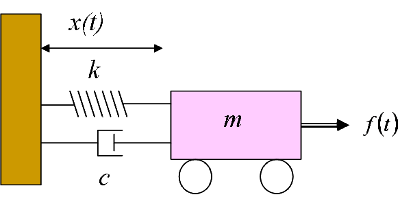
\includegraphics[width=\textwidth]{Images/SpringMassDamper_cartSystem.png}
				Spring Mass Damper System \cite{ctms_engin_umich_SystemModeling}
			\end{figure}
		\end{column}
	\end{columns}
	
	\footnotesize{
		Activity: 
		\url{https://www.sccs.swarthmore.edu/users/12/abiele1/Linear/examples/simple.html}
	}
\end{frame}
\subsection{Derivation: Transfer Function and Step-Response}
\begin{frame}
	\frametitle{Transfer Function Derivation}
	\textbf{Convert Differential Equation to Laplace:}
	\only<.>{(Assume: $x(t) = \dot{x}(t) = 0$)}
	\[
		f(t) = m \ddot{x}(t) + b \dot{x}(t) + k x(t)
		\visible<+-| alert@+>{
			\quad \overset{\mathcal{L}}{\Rightarrow} \quad
		F(s) = m s^2 X(s) + b s X(s) + k X(s)}
	\]
	\visible<+->{
		\textbf{Solve for $X(s)$ in terms of $F(s)$}
	\[
		F(s) = (ms^2 + b s + k) X(s)
	\]
	}
	\visible<+->{
	\[
		X(s) = 
		\alert<+>{\cfrac{1}{ms^2 + bs + k} F(s)}
		= \cfrac{\qty(\frac{k}{k})}{m(s^2+\frac{b}{m}s+\frac{k}{m})} F(s)
		= \cfrac{\frac{k}{m}}{s^2 + \frac{b}{m}s + \frac{k}{m}} \qty(\frac{1}{k}) F(s)
	\]}
	\visible<+->{
	\textbf{Transfer Function:}
	\[
		\visible<.(1)>{\underset{\textbf{(Hook's Law)}}{\alert{F = k \Delta x}}\Rightarrow}
		H(s) = \frac{X(s)}{F(s)} = \alert<+>{\qty(\frac{1}{k})}
		\alert<+>{\cfrac{\frac{k}{m}}{s^2 + \frac{b}{m} s + \frac{k}{m}}}
		\visible<.>{\Leftarrow 
			\underset{\textbf{(Standard Form)}}{
				\alert{\frac{\omega_0^2}{s^2 + 2\zeta\omega_0 s + \omega_0^2}}
			}
		}
	\]
	}
\end{frame}

\begin{frame}
	\frametitle{Factoring the characteristic polynomial}
	Apply the quadratic formula to find the roots of the characteristic polynomial:
	\[
		\Delta(s) 
		% = s^2 + \frac{b}{m} s + \frac{k}{m}
		= m s^2 + b s + k
		\quad \Rightarrow \quad
		s = \cfrac{-b \pm \sqrt{b^2 - 4mk}}{2m}
	\]
	\pause
	\textbf{3 Potential cases:} %(may have learned in differential equations)
	\begin{enumerate}[<+- | alert@+>]
		\item \textbf{Damped}: 
		$b^2 > 4mk \Rightarrow 
		p_1 \neq p_2 \Rightarrow (s+p_1)(s+p_2)$
		% p_1 = a, p_2 = b \Rightarrow (s+a)(s+b)$
		% $(\frac{b}{2m})^2 > \frac{k}{m} \Rightarrow (s+a)(s+b)$
		\item \textbf{Critically Damped}:
		\(
			b^2 = 4mk \Rightarrow p_1 = p_2 
			\Rightarrow {(s+p_{1,2})}^2
		\)
		% p_1 = p_2 = a \Rightarrow (s + a)^2$
		% $(\frac{b}{2m})^2 = \frac{k}{m} \Rightarrow (s + a)^2$
		\item \textbf{Underdamped}: 
		$b^2 < 4mk \Rightarrow p_{1,2} = \sigma \pm j \omega 
		$
		% \Rightarrow (s+\sigma +j\omega)(s + \sigma - j\omega)$
		% $(\frac{b}{2m})^2 < \frac{k}{m} \Rightarrow (s + \sigma \pm j \omega)$
	\end{enumerate}
	
	\note<+>{
	This motivates the standard characteristic polynomial form:
	\begin{align*}
		s^2 + 2 \zeta \omega_0 s + \omega_0^2
		\Rightarrow
		s = \zeta \omega_0 \pm \sqrt{(\zeta \omega_0)^2 - \omega_0^2}
		= \omega_0 \qty(\zeta \pm \sqrt{\zeta - 1})\\
		\intertext{Let $2 \zeta \omega_n = \sqrt{\frac{b}{m}}$ and $\omega_0 = \sqrt{\frac{k}{m}}$}
		\Delta(s) = s^2 + \frac{b}{m} s + \qty(\sqrt{\frac{k}{m}})^2
		\iff \Delta(s) = s^2 + 2\zeta \omega_0 s + \omega_0^2
	\end{align*}
	In this instance, the three cases are easily seen based on $\zeta$:
	\begin{enumerate}
		\item Damped: $\zeta > 1$
		\item Critically Damped: $\zeta = 1$
		\item Underdamped: $\zeta \in [0,1)$
	\end{enumerate}
	}
\end{frame}
% \begin{frame}
% 	\frametitle{Factoring the characteristic polynomial}
% 	Apply the quadratic formula to find the roots of the characteristic polynomial:
% 	\[
% 		\Delta(s) 
% 		% = s^2 + \frac{b}{m} s + \frac{k}{m}
% 		= m s^2 + b s + k
% 		\quad \Rightarrow \quad
% 		s = \cfrac{-b \pm \sqrt{b^2 - 4mk}}{2m}
% 	\]
% 	% $\Delta(s) = 0 = ms+^2+bs+k = s^2 + \frac{b}{m}s + \frac{k}{m}$.
% 	% In order to do the partial fraction decomposition, it must be in factored form, thus factoring via the quadratic equation: $\Delta(s) = m s^2 + b s + k$
% 	% \begin{align*}
% 	% 	s = \cfrac{-b \pm \sqrt{b^2 - 4mk}}{2m}
% 	% 	= -\frac{b}{2m} \pm \sqrt{\frac{b^2 -4mk}{4m^2}}
% 	% 	= -\frac{b}{2m} \pm \sqrt{\qty(\frac{b}{2m})^2 - \sqrt{\frac{k}{m}}^2}
% 	% \end{align*}
% 	\pause
% 	\textbf{3 Potential cases:} %(may have learned in differential equations)
% 	\begin{enumerate}[<+- | alert@+>]
% 		\item \textbf{Damped}: 
% 		$b^2 > 4mk \Rightarrow 
% 		p_1 \neq p_2 \Rightarrow (s+p_1)(s+p_2)$
% 		% p_1 = a, p_2 = b \Rightarrow (s+a)(s+b)$
% 		% $(\frac{b}{2m})^2 > \frac{k}{m} \Rightarrow (s+a)(s+b)$
% 		\item \textbf{Critically Damped}:
% 		\(
% 			b^2 = 4mk \Rightarrow p_1 = p_2 
% 			\Rightarrow {(s+p_{1,2})}^2
% 		\)
% 		% p_1 = p_2 = a \Rightarrow (s + a)^2$
% 		% $(\frac{b}{2m})^2 = \frac{k}{m} \Rightarrow (s + a)^2$
% 		\item \textbf{Underdamped}: 
% 		$b^2 < 4mk \Rightarrow p_{1,2} = \sigma \pm j \omega 
% 		$
% 		% \Rightarrow (s+\sigma +j\omega)(s + \sigma - j\omega)$
% 		% $(\frac{b}{2m})^2 < \frac{k}{m} \Rightarrow (s + \sigma \pm j \omega)$
% 	\end{enumerate}
	
% 	\note<+>{
% 	This motivates the standard characteristic polynomial form:
% 	\begin{align*}
% 		s^2 + 2 \zeta \omega_0 s + \omega_0^2
% 		\Rightarrow
% 		s = \zeta \omega_0 \pm \sqrt{(\zeta \omega_0)^2 - \omega_0^2}
% 		= \omega_0 \qty(\zeta \pm \sqrt{\zeta - 1})\\
% 		\intertext{Let $2 \zeta \omega_n = \sqrt{\frac{b}{m}}$ and $\omega_0 = \sqrt{\frac{k}{m}}$}
% 		\Delta(s) = s^2 + \frac{b}{m} s + \qty(\sqrt{\frac{k}{m}})^2
% 		\iff \Delta(s) = s^2 + 2\zeta \omega_0 s + \omega_0^2
% 	\end{align*}
% 	In this instance, the three cases are easily seen based on $\zeta$:
% 	\begin{enumerate}
% 		\item Damped: $\zeta > 1$
% 		\item Critically Damped: $\zeta = 1$
% 		\item Underdamped: $\zeta \in [0,1)$
% 	\end{enumerate}
% 	}
% \end{frame}




\subsection{Activity: Response Comparison}
\begin{frame}
	\frametitle{Case 1 (Damped)}
	% Let $a = \frac{b}{2m} + \sqrt{\qty(\frac{b}{2m})^2 - \qty(\sqrt{\frac{k}{m}})^2}$ and $b = \frac{b}{2m} - \sqrt{\qty(\frac{b}{2m})^2 - \qty(\sqrt{\frac{k}{m}})^2}$
	\begin{gather*}
		X(s) 
		= \cfrac{1}{m s (s^2 + \frac{b}{m}s + \frac{k}{m})}
		= \cfrac{\frac{1}{m}}{s(s+a)(s+b)}
		\intertext{
			Evaluate Coefficients:
			$C_{i} = \eval{\frac{(s-\lambda_{i})}{m (s(s+a)(s+b))}}_{s = \lambda_{i}}$
		}
		X(s) = \cfrac{C_1}{s} + \cfrac{C_2}{s+a} + \cfrac{C_3}{s+b}
		\overset{\mathcal{L}}{\iff}
		x(t) = \qty(C_1 + C_2 e^{-at} + C_3 e^{-bt}) u(t)
	\end{gather*}

	\note{
		% \[
		% 	C_{1,2,3} = \eval{\cfrac{\frac{1}{m}}{s(s+a)(s+b)}(s-\lambda_{i})}_{s = \lambda_{i}}
		% \]
		Evaluate coeficients:
		$(a)(b) = (\frac{b}{2m})^2 - ((\frac{b}{m})^2-\frac{k}{m}) = \frac{k}{m}$, \quad $(a-b) = 2\sqrt{(\qty(\frac{b}{2m})^2 - \frac{k}{m})}$
		\begin{gather*}
			C_1 = \eval{\frac{(s)}{m s(s+a)(s+b)}}_{s=0}
			= \frac{1}{m (a)(b)}
			\Rightarrow
			C_1 = \frac{1}{k} \textbf{(Hook's Law @ steady-state)}
			\\
			C_2 = \eval{\frac{(s+a)}{m s(s+a)(s+b)}}_{s=-a}
			= \frac{1}{m(-a)(-a+b)}
			= \frac{1}{m(a)(a-b)}
			\\
			C_3 = \eval{\frac{(s+b)}{m s(s+a)(s+b)}}_{s=-b}
			= \frac{1}{m(-b)(a-b)}
			= \frac{-1}{m(b)(a-b)}\\
			C_{2,3} = \cfrac{\pm 1}{2m\sqrt{(\qty(\frac{b}{2m})^2 - \frac{k}{m})} \qty(\frac{b}{2m} \pm \sqrt{\qty(\frac{b}{2m})^2 - \qty(\sqrt{\frac{k}{m}})^2})}
		\end{gather*}
	}
	
\end{frame}

\begin{frame}
	\frametitle{Case 2 (Critically Damped)}
	Let $a = \frac{b}{2m}$
	\begin{gather*}
		X(s) = \cfrac{\frac{1}{m}}{s (s+a)^2} 
		= \cfrac{C_1}{s} + \cfrac{C_2}{s+a} + \cfrac{C_3}{(s+a)^2}
		\overset{\mathcal{L}}{\Rightarrow}
		x(t) = \qty(C_1 + C_2 e^{-a t} + C_3 t e^{-a t}) u(t)
	\end{gather*}
\end{frame}

\begin{frame}
	\frametitle{Case 3 (Underdamped)}
	Let $\sigma = \frac{b}{m}$ and $\omega = \sqrt{\sqrt{\frac{k}{m}}^2 - \qty(\frac{b}{2m})^2}$
	
	\begin{align*}
		X(s) &= \cfrac{\frac{1}{m}}{s (s+\sigma \pm j\omega)} 
		= \cfrac{C_1}{s} + \cfrac{C_2}{(s+\sigma+j\omega)} + \cfrac{C_3}{(s+\sigma - j\omega)}\\
		& \qquad \Updownarrow \mathcal{L}\\
		% \overset{\mathcal{L}}{\Rightarrow}\\
		% \overset{\mathcal{L}}{\Rightarrow}
		x(t) &= \qty(C_1 + C_2 e^{-\sigma t}e^{j\omega t} + C_3 e^{-\sigma t} e^{-j\omega t}) u(t)\\
		&= C_1 u(t) + 2 e^{-\sigma t} u(t) \frac{C_2 e^{j\omega t} + C_3 e^{-j\omega t}}{2}
		\Leftarrow \textbf{Convert using Euler's Identity}
	\end{align*}
	

\note{
	Alternative approach
	\begin{align*}
		X(s) &= \cfrac{\frac{1}{m}}{s (s^2 + \frac{b}{m}s + \frac{k}{m})}
		= \cfrac{C_1}{s} + \cfrac{C_2}{(s+\frac{b}{2m})^2 + \sqrt{\frac{k}{m}-\sqrt{\frac{b}{m}}}^2}
		\overset{\mathcal{L}}{\Rightarrow}\\
		&\overset{\mathcal{L}}{\Rightarrow}
		x(t) = \qty(C_1 + \frac{C_2}{\sqrt{\frac{k}{m}-\sqrt{\frac{b}{m}}}} \exp{-\cfrac{b}{2m}t} \cos{\qty(\sqrt{\frac{k}{m}-\sqrt{\frac{b}{m}}})t}) u(t)
	\end{align*}
}

\end{frame}
% \note{	
% 	Characteristic Polynomial :\[
% 		\Delta(s)
% 		= m s^2 + b s + k
% 		\Rightarrow s^2 + \frac{b}{m} s + \frac{k}{m}
% 		% = s^2 + 2 \zeta \omega_0 s + \omega_0^2
% 	\]
% }



	
	% 2\textsuperscript{nd}-Order Dynamical System:
	% \[
	% 	\ddot{x}(t) + 2 \zeta \omega_0 \dot{x}(t) + \omega_0^2 x(t) = u(t)
	% \]


% \note{

% \begin{align*}
% 	m \ddot{x}(t) + b \dot{x}(t) + k x(t) &= f(t)\\
% 	&\Downarrow \mathcal{L}\\
% 	m s^2 X(s) + b s X(s) + k X(s) &= F(s)\\
% 	(m s^2 + bs + k) X(s) &= F(s)\\
% 	X(s) &= \frac{1}{ms^2 + b s + k} F(s)
% 	% s^2 X(s) + \frac{b}{m} s X(s) + \frac{k}{m} X(s) &= \frac{1}{m} F(s)\\
% 	% \qty(s^2 + \frac{b}{m} s + \frac{k}{m}) X(s) &= \frac{1}{m} F(s)\\
% 	% X(s) &= \cfrac{\frac{1}{m}}{s^2 + \frac{b}{m} s + \frac{k}{m}} F(s)\\
% 	% TODO: factor it here...
% \end{align*}
% Charectoristic Polynomial :\[
% 	\Delta(s)
% 	= m s^2 + b s + k
% 	\Rightarrow s^2 + \frac{b}{m} s + \frac{k}{m}
% 	= s^2 + 2 \zeta \omega_0 s + \omega_0^2
% \]

% } \note{

% In order to do the partial fraction decomposition, it must be in factored form... 
% thus the quadratic equation:
% \[
% 	\Delta(s) = m s^2 + b s + k = 0 
% 	\Rightarrow s 
% 	= \cfrac{-b \pm \sqrt{b^2 - 4mk}}{2m}
% 	= \frac{b}{2m} \pm \sqrt{\frac{b^2 -4mk}{4m^2}}
% 	= \frac{b}{2m} \pm \sqrt{\qty(\frac{b}{2m})^2 - \frac{k}{m}}
% \]

% 3 Potential cases: (may have learned in differential equations)
% \begin{enumerate}
% 	\item \textbf{Damped}: $(\frac{b}{2m})^2 > \frac{k}{m} \Rightarrow (s+a)(s+b)$
% 	\item \textbf{Critically Damped}:$(\frac{b}{2m})^2 = \frac{k}{m} \Rightarrow (s + a)^2$
% 	\item \textbf{Underdamped}: $(\frac{b}{2m})^2 < \frac{k}{m} \Rightarrow (s + \sigma \pm j \omega_d)$
% \end{enumerate}

% We will continue under the assumption that the system is underdamped and then return for a more general case.

% } 
% \note{

% Step Response: 
% $f(t) = u(t) \overset{\mathcal{L}}{\Rightarrow} F(s) = \frac{1}{s}$
% \begin{align*}
% 	X(s) 
% 	&= \cfrac{\frac{1}{m}}{s^2 + \frac{b}{m} s + \frac{k}{m}} \qty(\frac{1}{s})
% 	= \cfrac{\frac{1}{m}}{s(s^2 + \frac{b}{m} s + \frac{k}{m})}
% 	\\
% 	\intertext{
% 		Factored Form (quadratic formula):
% 	$a s^2 + b s + c = 0 \Rightarrow s = \cfrac{-b \pm \sqrt{b^2 - 4ac}}{2a}$
% 	}
% 	TODO: factor it... 3 cases...
% 	% X(s) &= \cfrac{\frac{1}{m}}{s (s + \cfrac{\frac{b}{m} \pm \sqrt{(\frac{b}{m})^2 - 4 \frac{k}{m}}}{2})}\\
% 	\intertext{Partial Fraction Expansion}
% 	X(s) &= 
% \end{align*}

% } \note{	

% Side Note: (skip unless time allows/go back to this)
% Looking at the original differential equation we can see how the standard form $s^2 + 2\zeta \omega_0 s + (\omega_0)^2$ would fit in as \[
% 	\zeta \omega_0 \pm \sqrt{(\zeta \omega_0)^2 - \omega_0^2}
% 	= \zeta \omega_0 \pm \sqrt{\omega_0^2 (\zeta^2 - 1)}
% 	= \zeta \omega_0 \pm \omega_0 \sqrt{\zeta^2 - 1}
% \]

% }










% \begin{frame}
% 	\frametitle{TLDR: Second-Order System Dynamics}
% 	\begin{columns}
% 		\begin{column}{0.5\textwidth}
% 			\textbf{Transfer Function}
% 			\[
% 				H(s) 
% 				= \cfrac{Y(s)}{U(s)} 
% 				= \cfrac{
% 					\omega_0^2
% 				}{
% 					s^2 + 2 \zeta \omega_0 s + \omega_0^2
% 				}
% 			\]
% 			\textbf{System Poles}
% 			\[
% 				s = - \zeta \omega_0 \pm \omega_0 \sqrt{1 - \zeta^2}
% 			\]
% 			\textbf{Spring Mass Damper System Parameters}
% 			\[
% 				\omega_0 = \sqrt{\cfrac{k}{m}}
% 				\hspace{0.5 in}
% 				\zeta = \sqrt{\cfrac{c^2}{4 m k}}
% 			\]
% 		\end{column}
% 		\begin{column}{0.375\textwidth}
% 			\begin{figure}[]
% 				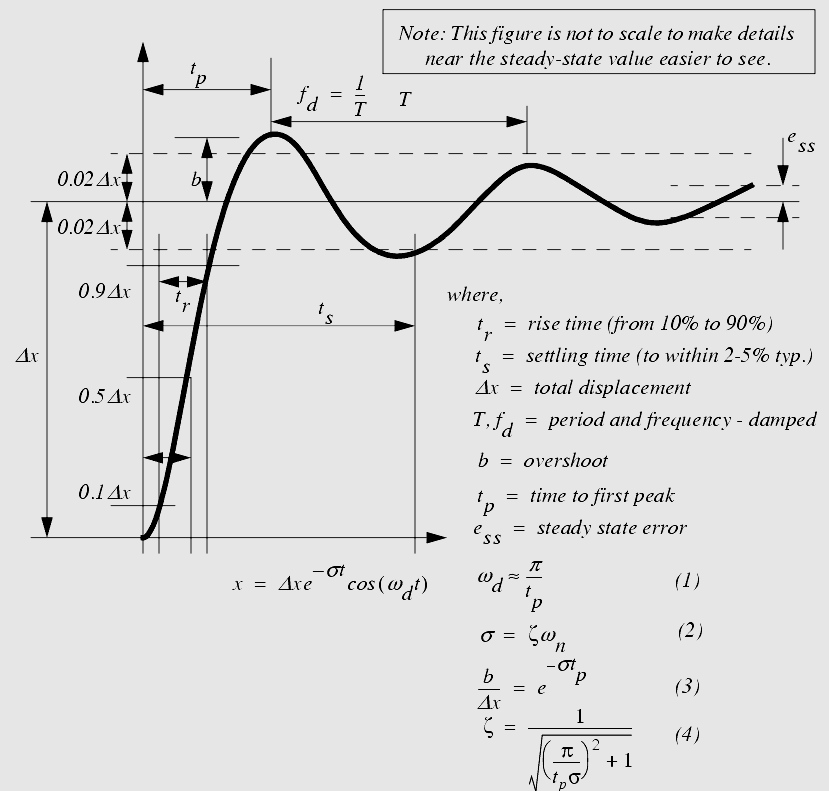
\includegraphics[width=\textwidth]{Images/2ndOrderTransient.png}
% 				2nd Order System Response \cite{engineerOnADisk_2ndOrderDynamics}
% 			\end{figure}
% 		\end{column}
% 	\end{columns}
% \end{frame}


\section*{}

\begin{frame}
	\frametitle{Lecture Overview}
	\[
		m \ddot{x}(t) + b \dot{x}(t) + k x(t) = f(t)
	\]
	\[
		X(s) = \frac{1}{m s^2 + b s + k} F(s) 
		= \frac{\frac{1}{m}}{s^2 + \frac{b}{m} s + \frac{k}{m}} F(s)
	\]
	\begin{columns}
		\begin{column}{0.5\textwidth}
			\[
				H(s) = \frac{X(s)}{U(s)}
				= \frac{
					\omega_0^2
				}{
					s^2 + 2 \zeta \omega_0 s + \omega_0^2
				}
			\]		
	\[
		\omega_0 = \sqrt{\frac{k}{m}}
		\quad
		\zeta = \sqrt{\frac{b^2}{4 m k}}
		\quad
		U(s) = \frac{1}{k} F(s)
	\]
			% \[
			% 	\omega_0 = \sqrt{\frac{k}{m}}
			% 	\quad
			% 	\zeta = \sqrt{\frac{c^2}{4 m k}}
			% \]
		\end{column}
		\begin{column}{0.25 \textwidth}
			\begin{figure}[]
				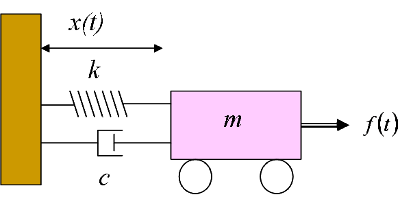
\includegraphics[width=\textwidth]{Images/SpringMassDamper_cartSystem.png}
			\end{figure}
		\end{column}
		% \begin{column}{0.3\textwidth}
		% 	\[
		% 		\color{red}
		% 		u(t) = U_0 \cos(\omega t)
		% 	\]
		% 	\[
		% 		\color{blue}
		% 		y(t) = Y_0 \cos(\omega t + \phi)
		% 	\]
		% 	\begin{figure}
		% 		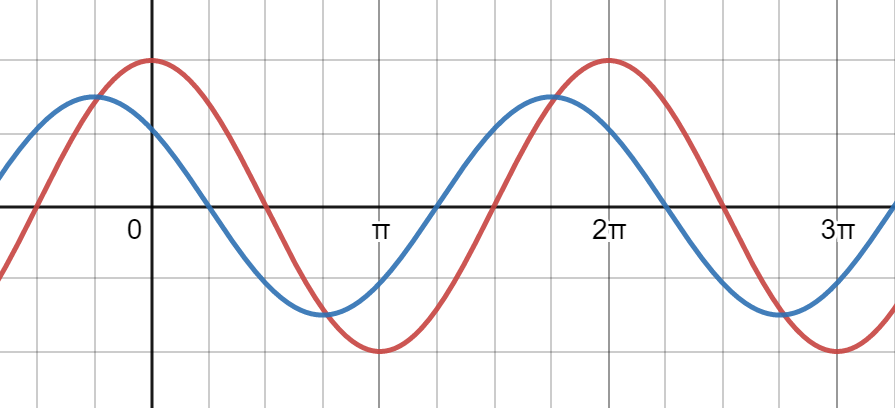
\includegraphics[width=\textwidth]{Images/phase_shift.png}
		% 	\end{figure}
		% \end{column}
		% \begin{column}{0.4\textwidth}
		% 	\begin{figure}
		% 		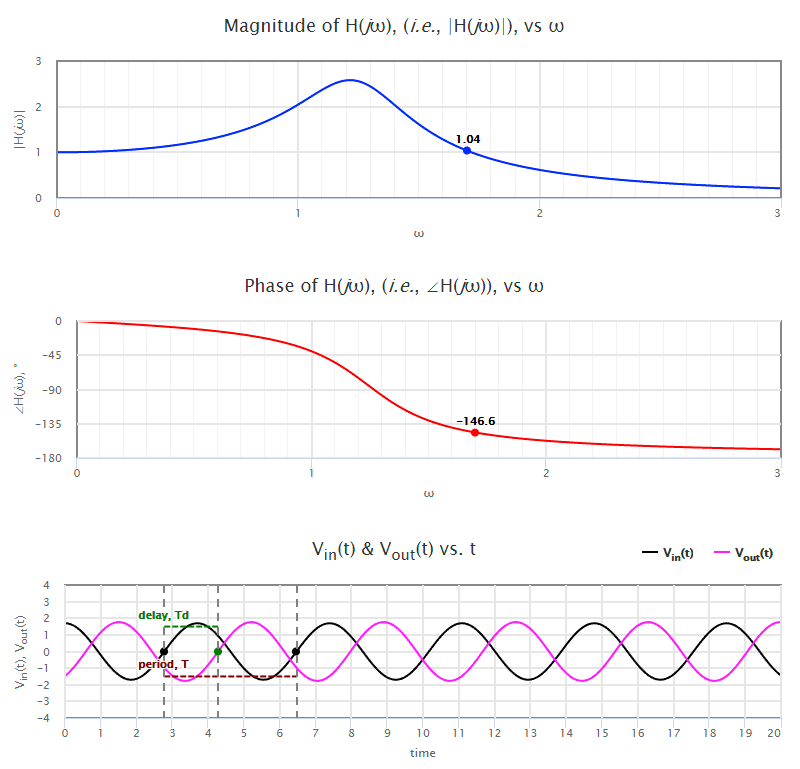
\includegraphics[width=\textwidth]{Images/bode_demo_2.png}
		% 	\end{figure}
		% \end{column}
	\end{columns}
\end{frame}


\begin{frame}[allowframebreaks]{Bibliography}
	\bibliographystyle{unsrt}
	\bibliography{refs}
\end{frame}



\begin{frame}
	\frametitle{TLDR: Second-Order System Dynamics}
	\begin{columns}
		\begin{column}{0.5\textwidth}
			\textbf{Transfer Function}
			\[
				H(s) 
				= \cfrac{Y(s)}{U(s)} 
				= \cfrac{
					\omega_0^2
				}{
					s^2 + 2 \zeta \omega_0 s + \omega_0^2
				}
			\]
			\textbf{System Poles}
			\[
				s = - \zeta \omega_0 \pm \omega_0 \sqrt{1 - \zeta^2}
			\]
			\textbf{Spring Mass Damper System Parameters}
			\[
				\omega_0 = \sqrt{\cfrac{k}{m}}
				\hspace{0.5 in}
				\zeta = \sqrt{\cfrac{c^2}{4 m k}}
			\]
		\end{column}
		\begin{column}{0.375\textwidth}
			\begin{figure}[]
				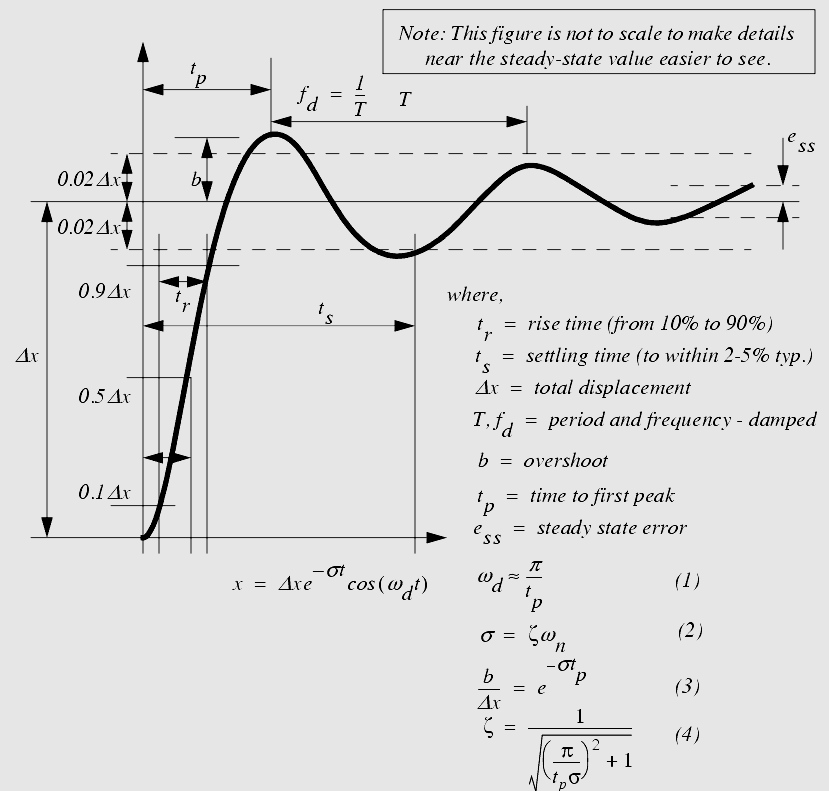
\includegraphics[width=\textwidth]{Images/2ndOrderTransient.png}
				2nd Order System Response \cite{engineerOnADisk_2ndOrderDynamics}
			\end{figure}
		\end{column}
	\end{columns}
\end{frame}

\end{document}